\documentclass[border=2pt]{standalone}

% Drawing
\usepackage{tikz}

\tikzset{>=latex}
\usetikzlibrary{decorations.markings, calc}

% New Command
%% Middle Line Label
\newcommand{\midlabelline}[3]{
   \node (midlabel) at ($ (#1)!.5!(#2) $) {#3};
   \draw[<-] (#1) --  (midlabel);
   \draw[->] (midlabel) -- (#2);
}
%% Point
\newcommand{\point}[3]{
\draw[fill=black] (#1) circle (1pt) node[#3] {#2};
}

% Styles
%% Arrow in the Middle
\tikzset{arrow inside/.style = {postaction=decorate,decoration={markings,mark=at position 0.52 with \arrow{stealth}}}}

% Define Color
\definecolor{glass}{cmyk}{0.2,0,0,0}

\begin{document}
	
	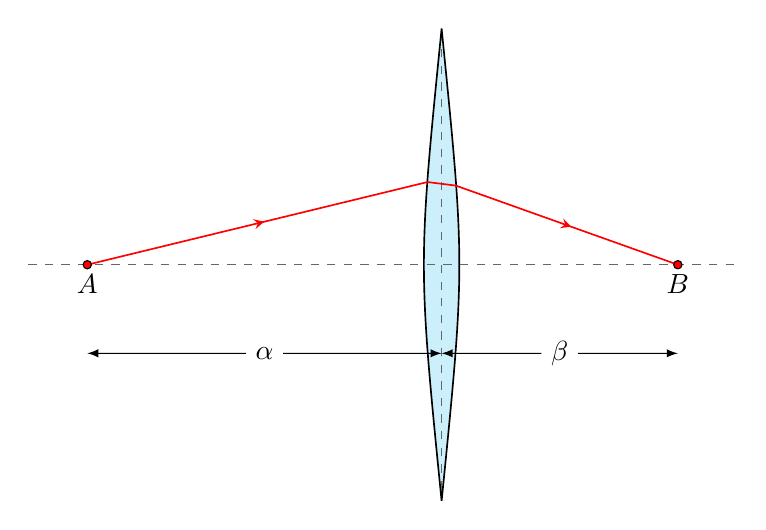
\begin{tikzpicture}[scale=1.5]
		% Grid
%		\draw[help lines] (-3,-3) grid (6,6);

		% Lens		
		\path[fill=glass, draw=black, line width = 0.6] (1,-2) .. controls (0.8,0) .. (1,2) .. controls (1.2,0) .. (1,-2);
		
		% Axis
		\draw[dashed, black!60] (1,-1.9) -- (1,1.9);
		\draw[dashed, black!60] (-2.5,0) -- (3.5,0);
		
		% Ray
		\draw[red, line width = 0.6, arrow inside] (-2,0) -- (0.88,0.7);	
		\draw[red, line width = 0.6] (0.88,0.7) -- (1.12,0.67);
		\draw[red, line width = 0.6, arrow inside] (1.12,0.67) -- (3.,0);
		
		%Points
		\draw[fill=red] (-2,0) circle (1pt) node[below] {$A$};
		\draw[fill=red] (3,0) circle (1pt) node[below] {$B$};
		
		% Distances
		\midlabelline{-2,-0.75}{1,-0.75}{$\alpha$}
		\midlabelline{1,-0.75}{3,-0.75}{$\beta$}
	\end{tikzpicture}
	
\end{document}